\documentclass{article}

\usepackage{jacksonmath}
\usepackage[english]{babel}
\usepackage[utf8]{inputenc}
\usepackage[final]{pdfpages}

\begin{document}
  \section{2.10 Problems 9, 10, 12}
  \begin{enumerate}
    \item[9] In order for \~ to be an equivalence relation it must be  symmetric, reflexive, and transitive.\\
      Reflexive: We can create a path $\gamma:[a,b]\to S$ defined as $\gamma(t)=z$. Clearly $\gamma$ connects z to itself so it is reflexive.\\
      Symmetry: If we have a path $\gamma(t)$ that connects $z,w$ then we also have a path $\gamma(-t)$ that connects $w,z$.\\
      Transitive: If we let $\gamma:[a,b]\to S$ and $\beta:[b,c]\to S$ connect $x,y$ and $y,z$. We can connect these paths to form a new path that goes from $x,z$ because we can combine paths. Thus it is transitive.\\
      A component will be non empty if there is at least 2 path connected points in $S$. Suppose we have a component $U\subseteq S$, we can see it is path connected by our previous work. Let's choose an arbitrary $z\in U$, but at the same time $z\in S$. This means we have $N_\epsilon(z)\subseteq S$, which is an open path connected disk. This means that $N_\epsilon(z)\subseteq U$ because $z$ connects to everything in the neighborhood and in $U$.
    \item[10] We need to show that for any two $z_1,z_2\in f(S)$, there  exists a path between them.\\
      We know there exists $z_1',z_2'\in S\st f(z_1')=z_1, f(z_2')=z_2$. There is a path $\gamma:[a,b]\to S$ in $S$ that connects them. The composition of two continuous functions is continuous so we have $f\odot\gamma$ connecting $z_1',z_2'$, thus $f$ connects $z_1,z_2$
    \item[12]
      \begin{enumerate}[label=\roman*]
        \item
          This set is clearly a ring. The boundary set would be   circles with the inner and outer radius. The set is not path connected because you cannot move from one circle to the other.\\
          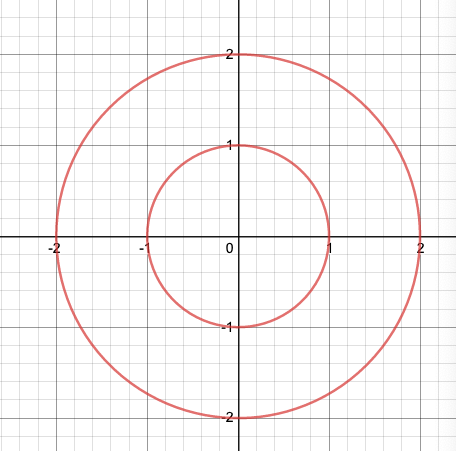
\includegraphics[scale=0.5]{graphs/i}
        \item
          The set $S$ consists of all points that are non zero. Thus the only limit point would be zero because it's neighborhood is in both $S$ and $\C\backslash S$ for any $\epsilon>0$. This would be path connected because there is only one point.\\
          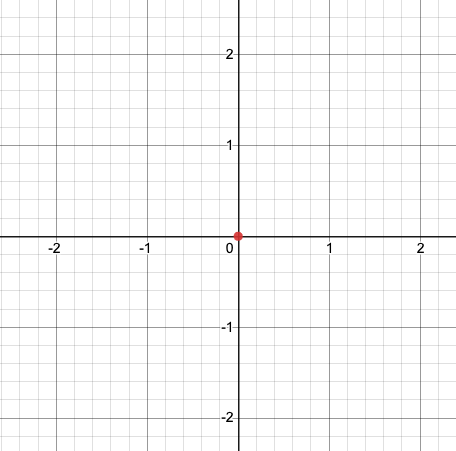
\includegraphics[scale=0.5]{graphs/ii}
        \item
          If we choose any point from the complex plane it is a limit point. If we choose some point $z$ then for any $\epsilon>0$ there exists a neighborhood with an infinite amount of rational numbers, but also an infinite number of non rationals. Thus the boundary is all points in $\C$. All of $\C$ is path connected.\\
          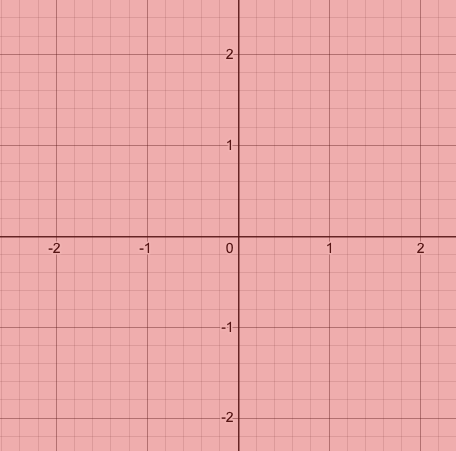
\includegraphics[scale=0.5]{graphs/iii}
        \item
          Any point inside the sqaure would be a limit point of only $S$, and any point outside would be a limit point for $\C\backslash S$. However, points on the edge of the square have neighborhoods containing points in $S$ and $\C\backslash S$ for any $\epsilon>0$. This is itself a path so all points are immediatley path connected.\\
          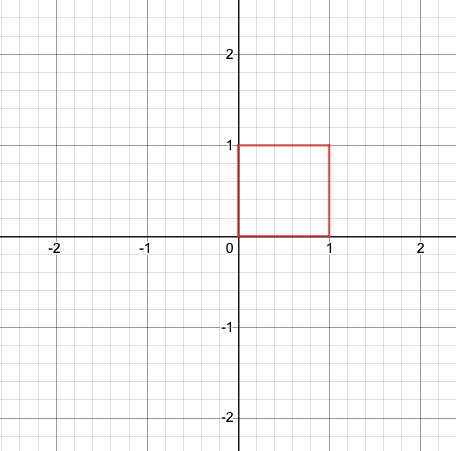
\includegraphics[scale=0.5]{graphs/iv}
        \item
          This set is all rational numbers in the unit square. If we take a rational number inside the square then it is a limit point like in (iii). If we take a point on the edge it is a limit point for the same reason. This square is also path connected because it is the unit square.\\
          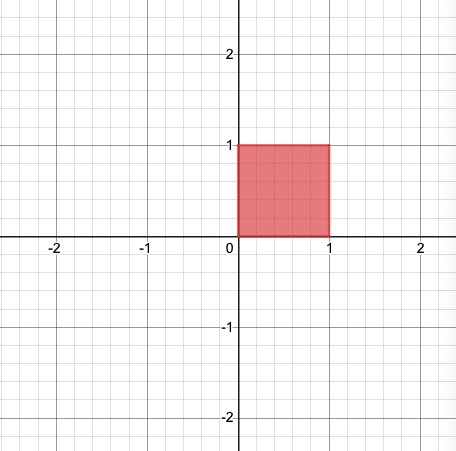
\includegraphics[scale=0.5]{graphs/v}
        \item
          Any point in the complex plane that is not on the negative imaginary axis. Thus the limit points must be on the negative imaginary axis. 0 is not in the set as well so it is a limit point. This is a path so it is path connected.\\
          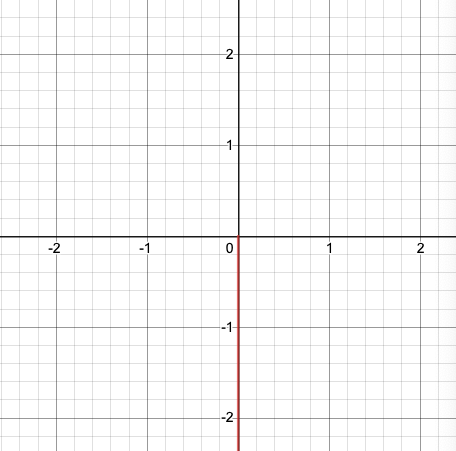
\includegraphics[scale=0.5]{graphs/vi}
        \item
          If we take the intersection of (ii) and (vi) we get the same set as in (vi), because (ii) contains all points besides zero and (vi) contains all points besides zero and those resting on the negative imaginary axis. Thus the answer is the same as (vi). It is path connected.\\
          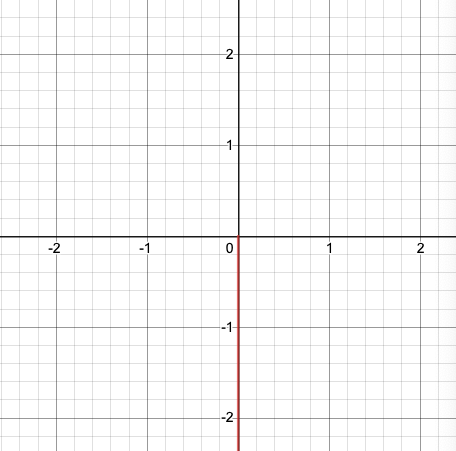
\includegraphics[scale=0.5]{graphs/vi}
      \end{enumerate}
  \end{enumerate}
  \section{3.6 Problems 2, 9, 10, 11}
  \begin{enumerate}
    \item[2] For which $z$ does the sequence converge?\\
      \begin{enumerate}[label=\roman*]
        \item $(z^n)$\\
          This will converge if $|z|\leq1$ because $|z^n|=|z|^n$.
        \item $(z^n/n)$\\
          This series will converge when $|z|\leq1$. This is the same as the last case.
        \item $(n!z^n)$\\
          \begin{align*}
            \lim_{n\to\infty}\frac{(n+1)!z^{n+1}}{n!z^n}=\lim_{n\to\infty}(n+1)z\\
          \end{align*}
          This limit will only converge when $z=0$. Otherwise it will go to $\infty$, because there is a some $n+1$ bigger than any $z$.
        \item $(z^n/n!)$\\
          \begin{align*}
            \left|\frac{z^{n+1}n!}{z^n(n+1)!}\right|=\left|\frac{z}{n+1}\right|
          \end{align*}
          this will converge for any $z$.
        \item
          \begin{align*}
            \left|\frac{z^{n+1}n^k}{z^n(n+1)^k}\right|&=\left|\frac{zn^k}{(n+1)^k}\right|\\
          \end{align*}
          Looking at this result we can see that it converges when $|z|\leq1$
        \item
          If we perform the ratio test this example becomes much easier.
          \begin{align*}
            \left|\frac{(a(a-1)...(a-n+1))z^{n+1}n!}{(a(a-1)...(a-n+1))(n+1)!z^n}\right|&=\left|\frac{z^{n+1}n!}{(n+1)!z^n}\right|\\&=\left|\frac{z}{n+1}\right|
          \end{align*}
          This is the same as (iv) so it converges for any $z$
      \end{enumerate}
    \item[9] Show that $\sum_{n=1}^\infty z^{n!}$ converges when $|z|<1$, but diverges for all $|z|=1$\\
      We will perform the ratio test on this series.
      \begin{align*}
        \lim_{n\to\infty}\left|\frac{z^{(n+1)!}}{z^{n!}}\right|&=\lim_{n\to\infty}\left|z^{(n+1)n!-n!}\right|\\
        &=\lim_{n\to\infty}|z^{n(n!)}|
      \end{align*}
      This limit will only be less than 1 when $|z|<1$. If we let $|z|=1$, then we get the series
      \begin{align*}
        \sum_{n=1}^\infty z^{n!}&=\sum_{n=1}^\infty(\cos\theta+i\sin\theta)^{n!}\\
        &=\sum_{n=1}^\infty \cos(n!\theta)+\sum_{n=1}^\infty i\sin(n!\theta)
      \end{align*}
      These series both oscillate so the series does not converge when $|z|=1$
    \item[10] $\sum a_nz^n$ has radius of convergence R, C is a circle of raius $R$.
      \begin{enumerate}[label=(\roman*)]
        \item if $\sum a_nz^n$ converges for some point on C then it converges for all points on C.\\
          Suppose $a_n=1/n$, giving us the series $\sum z^n/n$. This will converge for the value $z=-1$, but not at $z=1$
        \item if $\sum a_nz^n$ converges absolutely then everwhere in C converges absolutely.\\
          We know this series converges
          \begin{align*}
            \sum |a_n||z^n|=\sum |a_n||z|^n
          \end{align*}
          when z equals some point we will call $z_1$. We can see for any $(z'\in C)(|z'|=R=|z_1|)$ so
          \[\sum |a_n||z_1|^n=\sum |a_n||z'|^n\]
          Thus the series converges absolutely for any value of $z$.
        \item if $\sum a_nz^n$ converges at every point except possible one in C, then it converges absolutely everwhere on C.\\
          Suppose we have the series
          \[\sum (-1)^nz^n/n=\sum (-1)^n(x+iy)^n/n\]
          This is an alternating series except when $z=-1$. This series never converges absolutely because $\sum |z|^n/n$ does not converge.
      \end{enumerate}
    \item[11] If $\sum a_nz^n$ has radius of convergence R, use the formula $1/R=\lim\sup|a_n|^{1/n}$\\
      \begin{enumerate}[label=(\roman*)]
        \item $\sum n^3a_nz^n$\\
          \begin{align*}
            1/R'&=\lim\sup|n^3a_n|^{1/n}\\
            &=\lim\sup|n^3|^{1/n}|a_n|^{1/n}\\
            &=\frac{\lim\sup|n|^{3/n}}{R}\\
            &=\frac{\lim\sup e^{3/n\cdot ln(|n|)}}{R}\\
            &=1/R
          \end{align*}
          So they have the same radius of convergence.
        \item $\sum a_n(z^3)^{n}$\\
          We have a radius of convergence $R$ for the original series. If we substitute instead $z^3$ then the series will converge when $|z^3|<R\implies|z|<R^{1/3}$. So the radius of convergence would be $R^{1/3}$.
        \item $\sum a_n^3z^n$\\
          \begin{align*}
            1/R'&=\lim\sup|a_n^3|^{1/n}\\
            &=\lim\sup|a_n|^{3/n}\\
            &=\lim\sup|a_n|^{1/n}\cdot|a_n|^{1/n}\cdot|a_n|^{1/n}\\
            &=\frac{1}{R^3}
          \end{align*}
      \end{enumerate}
  \end{enumerate}
\end{document}
